\documentclass[11pt,a4paper]{article}

% =========================================================================
% PAKET-PAKET UTAMA
% =========================================================================
\usepackage[utf8]{inputenc}
\usepackage[T1]{fontenc}
\usepackage{lmodern}
\usepackage[indonesian]{babel}
\usepackage{amsmath,amssymb,amsfonts,amsthm}
\usepackage{bm}              % Notasi tebal untuk vektor & matriks
\usepackage{geometry}
\geometry{top=2.5cm, bottom=2.5cm, left=2.5cm, right=2.5cm}
\usepackage{graphicx}
\usepackage{booktabs}        % Tabel profesional
\usepackage{tabularx}
\usepackage{microtype}
\usepackage{xcolor}
\usepackage{mdframed}        % Kotak highlight untuk definisi
\usepackage{caption}
\usepackage{subcaption}
\usepackage{float}
\usepackage{tikz}
\usetikzlibrary{shapes.geometric, arrows.meta, positioning, calc}
\usepackage{hyperref}
\hypersetup{
    colorlinks=true,
    linkcolor=blue!70!black,
    citecolor=blue!70!black,
    urlcolor=blue!70!black,
    pdfencoding=auto,
    psdextra
}
\pdfstringdefDisableCommands{%
  \def\boldsymbol#1{#1}%
  \def\bm#1{#1}%
  \def\mathbf#1{#1}%
}

% Makro sitasi fleksibel
\newcommand{\citep}[2][]{(Rasmussen \& Williams, 2006\if\relax\detokenize{#1}\relax\else, #1\fi)}
\newcommand{\citet}[2][]{Rasmussen \& Williams (2006\if\relax\detokenize{#1}\relax\else, #1\fi)}

% Lingkungan Teorema & Definisi
\newtheorem{definisi}{Definisi}[section]
\newtheorem{teorema}{Teorema}[section]
\newtheorem{catatan}{Catatan}[section]

% Path direktori gambar
\graphicspath{{figures/}}

% =========================================================================
% INFORMASI DOKUMEN
% =========================================================================
\title{
    \vspace{-1.2cm}
    \textbf{\Large BIMBINGAN TUGAS AKHIR \#5} \\[0.2em]
}
\author{}
\date{Jumat, 9 Oktober 2026}

\begin{document}

\maketitle
\vspace{-0.8cm}

% =========================================================================
% 1. CONTOH PERHITUNGAN NUMERIK OPTIMASI HYPERPARAMETER (GRADIENT DESCENT 2x2)
% =========================================================================
\section{Contoh Perhitungan Optimasi Log Marginal Likelihood (\texorpdfstring{$2 \times 2$}{2 x 2})}
\label{sec:contoh_perhitungan_2x2}
\noindent \textit{\citep[Bab~5.4.1, hlm.~113--114, Persamaan~(5.9)]{rasmussen2006gaussian}}

\begin{equation}
\frac{\partial \log p(\mathbf{y}|X, \boldsymbol{\theta})}{\partial \theta_j} = \frac{1}{2} \operatorname{tr}\left( \left( \boldsymbol{\alpha}\boldsymbol{\alpha}^T - K_y^{-1} \right) \frac{\partial K_y}{\partial \theta_j} \right), \quad \text{dengan } \boldsymbol{\alpha} = K_y^{-1}\mathbf{y} \label{eq:rasmussen_5_9}
\end{equation}

\noindent Karena algoritma optimasi (seperti \textit{Gradient Descent} maupun \textit{Adam}) bertujuan untuk meminimumkan suatu fungsi objektif sedangkan tujuan kita adalah memaksimumkan \textit{log marginal likelihood}, maka fungsi objektif yang diminimumkan dikalikan $-1$ ($-\log p(\mathbf{y}|X, \boldsymbol{\theta})$):
\begin{equation}
-\frac{\partial \log p(\mathbf{y}|X, \boldsymbol{\theta})}{\partial \theta_j} = -\frac{1}{2} \operatorname{tr}\left( \left( \boldsymbol{\alpha}\boldsymbol{\alpha}^T - K_y^{-1} \right) \frac{\partial K_y}{\partial \theta_j} \right)
\end{equation}

\begin{figure}[H]
\centering
\begin{tikzpicture}[
    node distance=0.65cm,
    startstop/.style={rectangle, rounded corners=5pt, minimum width=5.2cm, minimum height=0.7cm, text centered, draw=blue!70!black, fill=blue!8, font=\small},
    process/.style={rectangle, rounded corners=3pt, minimum width=6.2cm, minimum height=0.7cm, text centered, draw=gray!70!black, fill=gray!8, font=\small},
    decision/.style={diamond, aspect=2.4, minimum width=4.0cm, minimum height=0.75cm, text centered, draw=orange!80!black, fill=orange!10, font=\footnotesize},
    arrow/.style={-{Stealth[length=2.5mm]}, thick, draw=blue!70!black},
    line/.style={thick, draw=blue!70!black}
]

% Nodes
\node (init) [startstop] {$\boldsymbol{\theta}^{(0)} = \begin{bmatrix} (\sigma_f^2)^{(0)} & \ell^{(0)} & (\sigma_n^2)^{(0)} \end{bmatrix}^T, \; t = 0, \; \eta, \; \mathbf{m}^{(0)} = \mathbf{0}, \; \mathbf{v}^{(0)} = \mathbf{0}, \; \beta_1, \; \beta_2, \; \epsilon$};
\node (ky) [process, below=of init] {$K_y = K_f(\boldsymbol{\theta}^{(t)}) + \sigma_n^2 I_n$};
\node (inv) [process, below=of ky] {$K_y^{-1}, \quad \boldsymbol{\alpha} = K_y^{-1}\mathbf{y}$};
\node (diff) [process, below=of inv] {$\boldsymbol{\alpha}\boldsymbol{\alpha}^T - K_y^{-1}$};
\node (grad) [process, below=of diff] {$-\nabla_{\boldsymbol{\theta}} \log p(\mathbf{y}|X, \boldsymbol{\theta}) = -\frac{1}{2} \operatorname{tr}\left( (\boldsymbol{\alpha}\boldsymbol{\alpha}^T - K_y^{-1}) \frac{\partial K_y}{\partial \boldsymbol{\theta}} \right)$};
\node (update) [process, below=of grad] {$\boldsymbol{\theta}^{(t+1)} = \boldsymbol{\theta}^{(t)} - \eta \left( -\nabla_{\boldsymbol{\theta}} \log p(\mathbf{y}|X, \boldsymbol{\theta}) \right) \quad \text{atau} \quad \boldsymbol{\theta}^{(t+1)} = \boldsymbol{\theta}^{(t)} - \eta \, \frac{\hat{\mathbf{m}}^{(t)}}{\sqrt{\hat{\mathbf{v}}^{(t)}} + \epsilon}$};
\node (dec) [decision, below=0.65cm of update] {$\|\boldsymbol{\theta}^{(t+1)} - \boldsymbol{\theta}^{(t)}\| < \text{tol}$ atau $t \ge T_{\max}$?};
\node (stop) [startstop, below=0.65cm of dec] {$\boldsymbol{\theta}^* = \boldsymbol{\theta}^{(t+1)}$};

% Arrows
\draw [arrow] (init) -- (ky);
\draw [arrow] (ky) -- (inv);
\draw [arrow] (inv) -- (diff);
\draw [arrow] (diff) -- (grad);
\draw [arrow] (grad) -- (update);
\draw [arrow] (update) -- (dec);
\draw [arrow] (dec) -- node[right, font=\footnotesize] {Ya} (stop);

% Looping Arrow back to ky
\draw [line] (dec.west) -- node[above, font=\footnotesize] {Tidak} ++(-2.4cm, 0) coordinate (loopleft);
\draw [line] (loopleft) -- node[left, font=\footnotesize] {$t \leftarrow t + 1$} (loopleft |- ky);
\draw [arrow] (loopleft |- ky) -- (ky.west);

\end{tikzpicture}
\caption{Diagram Iterasi Optimasi Hyperparameter.}
\label{fig:diagram_iterasi_gp}
\end{figure}

\subsection{Gradient Descent}
\label{subsec:gradient_descent}

\subsubsection*{1. Data Observasi \& Parameter Awal}
\begin{itemize}
    \item Data Input: $X = \begin{bmatrix} x_1 \\ x_2 \end{bmatrix} = \begin{bmatrix} 0 \\ 1 \end{bmatrix}$, \quad Target: $\mathbf{y} = \begin{bmatrix} y_1 \\ y_2 \end{bmatrix} = \begin{bmatrix} 1 \\ 2 \end{bmatrix}$
    \item Jarak: $r_{12} = |x_1 - x_2| = 1 \implies r_{12}^2 = (x_1 - x_2)^2 = 1$
    \item Kernel RBF: $k(x_p, x_q) = \sigma_f^2 \exp\left(-\frac{r_{pq}^2}{2\ell^2}\right)$
    \item Inisialisasi: $\boldsymbol{\theta}^{(0)} = \begin{bmatrix} (\sigma_f^2)^{(0)} \\ \ell^{(0)} \\ (\sigma_n^2)^{(0)} \end{bmatrix} = \begin{bmatrix} 1{,}0 \\ 1{,}0 \\ 0{,}1 \end{bmatrix}$, \quad Learning Rate: $\eta = 0{,}1$
\end{itemize}

\subsubsection*{2. Matriks Kovariansi \texorpdfstring{$K_y$}{Ky}}
\begin{align}
k_{11} &= k_{22} = \sigma_f^2 = 1{,}0 \\
k_{12} &= k_{21} = 1{,}0 \cdot \exp\left(-\frac{1}{2(1{,}0)^2}\right) = e^{-0{,}5} \approx 0{,}6065 \\
K_y &= \begin{bmatrix} \sigma_f^2 + \sigma_n^2 & k_{12} \\ k_{21} & \sigma_f^2 + \sigma_n^2 \end{bmatrix} = \begin{bmatrix} 1{,}0 + 0{,}1 & 0{,}6065 \\ 0{,}6065 & 1{,}0 + 0{,}1 \end{bmatrix} = \begin{bmatrix} 1{,}1000 & 0{,}6065 \\ 0{,}6065 & 1{,}1000 \end{bmatrix}
\end{align}

\subsubsection*{3. Determinan, Invers \texorpdfstring{$K_y^{-1}$}{Ky^(-1)}, dan Vektor \texorpdfstring{$\boldsymbol{\alpha}$}{alpha}}
\begin{align}
|K_y| &= (1{,}1000)^2 - (0{,}6065)^2 = 1{,}2100 - 0{,}3678 = 0{,}8422 \\
K_y^{-1} &= \frac{1}{0{,}8422} \begin{bmatrix} 1{,}1000 & -0{,}6065 \\ -0{,}6065 & 1{,}1000 \end{bmatrix} = \begin{bmatrix} 1{,}3062 & -0{,}7202 \\ -0{,}7202 & 1{,}3062 \end{bmatrix} \\
\boldsymbol{\alpha} &= K_y^{-1} \mathbf{y} = \begin{bmatrix} 1{,}3062 & -0{,}7202 \\ -0{,}7202 & 1{,}3062 \end{bmatrix} \begin{bmatrix} 1 \\ 2 \end{bmatrix} = \begin{bmatrix} (1{,}3062)(1) + (-0{,}7202)(2) \\ (-0{,}7202)(1) + (1{,}3062)(2) \end{bmatrix} = \begin{bmatrix} -0{,}1342 \\ 1{,}8922 \end{bmatrix}
\end{align}

\subsubsection*{4. Matriks \texorpdfstring{$(\boldsymbol{\alpha}\boldsymbol{\alpha}^T - K_y^{-1})$}{(alpha alpha^T - Ky^(-1))}}
\begin{align}
\boldsymbol{\alpha}\boldsymbol{\alpha}^T &= \begin{bmatrix} -0{,}1342 \\ 1{,}8922 \end{bmatrix} \begin{bmatrix} -0{,}1342 & 1{,}8922 \end{bmatrix} \nonumber \\
&= \begin{bmatrix} (-0{,}1342)^2 & (-0{,}1342)(1{,}8922) \\ (1{,}8922)(-0{,}1342) & (1{,}8922)^2 \end{bmatrix} = \begin{bmatrix} 0{,}0180 & -0{,}2540 \\ -0{,}2540 & 3{,}5805 \end{bmatrix} \\
\boldsymbol{\alpha}\boldsymbol{\alpha}^T - K_y^{-1} &= \begin{bmatrix} 0{,}0180 & -0{,}2540 \\ -0{,}2540 & 3{,}5805 \end{bmatrix} - \begin{bmatrix} 1{,}3062 & -0{,}7202 \\ -0{,}7202 & 1{,}3062 \end{bmatrix} = \begin{bmatrix} -1{,}2882 & 0{,}4662 \\ 0{,}4662 & 2{,}2743 \end{bmatrix}
\end{align}

\subsubsection*{5. Perhitungan Gradien}

\paragraph*{a. Terhadap \texorpdfstring{$\sigma_f^2$}{sigma_f^2}:}
\begin{align}
\frac{\partial K_y}{\partial \sigma_f^2} &= \begin{bmatrix} 1 & 0{,}6065 \\ 0{,}6065 & 1 \end{bmatrix} \\
\left( \boldsymbol{\alpha}\boldsymbol{\alpha}^T - K_y^{-1} \right) \frac{\partial K_y}{\partial \sigma_f^2} &= \begin{bmatrix} -1{,}2882 & 0{,}4662 \\ 0{,}4662 & 2{,}2743 \end{bmatrix} \begin{bmatrix} 1 & 0{,}6065 \\ 0{,}6065 & 1 \end{bmatrix} = \begin{bmatrix} -1{,}0054 & -0{,}3151 \\ 1{,}8456 & 2{,}5570 \end{bmatrix} \\
\operatorname{tr}\left( \left( \boldsymbol{\alpha}\boldsymbol{\alpha}^T - K_y^{-1} \right) \frac{\partial K_y}{\partial \sigma_f^2} \right) &= -1{,}0054 + 2{,}5570 = 1{,}5516 \\
\frac{\partial \log p(\mathbf{y}|X, \boldsymbol{\theta})}{\partial \sigma_f^2} &= \frac{1}{2} (1{,}5516) = 0{,}7758 \implies -\frac{\partial \log p(\mathbf{y}|X, \boldsymbol{\theta})}{\partial \sigma_f^2} = -0{,}7758
\end{align}

\paragraph*{b. Terhadap \texorpdfstring{$\ell$}{l}:}
\begin{align}
\frac{\partial K_y}{\partial \ell} &= \begin{bmatrix} 0 & 0{,}6065 \cdot \frac{r_{12}^2}{1^3} \\ 0{,}6065 \cdot \frac{r_{12}^2}{1^3} & 0 \end{bmatrix} = \begin{bmatrix} 0 & 0{,}6065 \\ 0{,}6065 & 0 \end{bmatrix} \\
\left( \boldsymbol{\alpha}\boldsymbol{\alpha}^T - K_y^{-1} \right) \frac{\partial K_y}{\partial \ell} &= \begin{bmatrix} -1{,}2882 & 0{,}4662 \\ 0{,}4662 & 2{,}2743 \end{bmatrix} \begin{bmatrix} 0 & 0{,}6065 \\ 0{,}6065 & 0 \end{bmatrix} = \begin{bmatrix} 0{,}2828 & -0{,}7813 \\ 1{,}3794 & 0{,}2828 \end{bmatrix} \\
\operatorname{tr}\left( \left( \boldsymbol{\alpha}\boldsymbol{\alpha}^T - K_y^{-1} \right) \frac{\partial K_y}{\partial \ell} \right) &= 0{,}2828 + 0{,}2828 = 0{,}5656 \\
\frac{\partial \log p(\mathbf{y}|X, \boldsymbol{\theta})}{\partial \ell} &= \frac{1}{2} (0{,}5656) = 0{,}2828 \implies -\frac{\partial \log p(\mathbf{y}|X, \boldsymbol{\theta})}{\partial \ell} = -0{,}2828
\end{align}

\paragraph*{c. Terhadap \texorpdfstring{$\sigma_n^2$}{sigma_n^2}:}
\begin{align}
\frac{\partial K_y}{\partial \sigma_n^2} &= \begin{bmatrix} 1 & 0 \\ 0 & 1 \end{bmatrix} = I_2 \\
\left( \boldsymbol{\alpha}\boldsymbol{\alpha}^T - K_y^{-1} \right) \frac{\partial K_y}{\partial \sigma_n^2} &= \begin{bmatrix} -1{,}2882 & 0{,}4662 \\ 0{,}4662 & 2{,}2743 \end{bmatrix} \\
\operatorname{tr}\left( \left( \boldsymbol{\alpha}\boldsymbol{\alpha}^T - K_y^{-1} \right) \frac{\partial K_y}{\partial \sigma_n^2} \right) &= -1{,}2882 + 2{,}2743 = 0{,}9861 \\
\frac{\partial \log p(\mathbf{y}|X, \boldsymbol{\theta})}{\partial \sigma_n^2} &= \frac{1}{2} (0{,}9861) = 0{,}4930 \implies -\frac{\partial \log p(\mathbf{y}|X, \boldsymbol{\theta})}{\partial \sigma_n^2} = -0{,}4930
\end{align}

\subsubsection*{6. Update Parameter}
\begin{align}
\nabla_{\boldsymbol{\theta}} \left( -\log p(\mathbf{y}|X, \boldsymbol{\theta}) \right) &= \begin{bmatrix} -\frac{\partial \log p(\mathbf{y}|X, \boldsymbol{\theta})}{\partial \sigma_f^2} \\[0.4em] -\frac{\partial \log p(\mathbf{y}|X, \boldsymbol{\theta})}{\partial \ell} \\[0.4em] -\frac{\partial \log p(\mathbf{y}|X, \boldsymbol{\theta})}{\partial \sigma_n^2} \end{bmatrix} = \begin{bmatrix} -0{,}7758 \\ -0{,}2828 \\ -0{,}4930 \end{bmatrix} \\
\boldsymbol{\theta}^{(1)} &= \boldsymbol{\theta}^{(0)} - \eta \, \nabla_{\boldsymbol{\theta}} \left( -\log p(\mathbf{y}|X, \boldsymbol{\theta}) \right) \\
\begin{bmatrix} (\sigma_f^2)^{(1)} \\[0.4em] \ell^{(1)} \\[0.4em] (\sigma_n^2)^{(1)} \end{bmatrix} &= \begin{bmatrix} 1{,}0000 \\ 1{,}0000 \\ 0{,}1000 \end{bmatrix} - 0{,}1 \begin{bmatrix} -0{,}7758 \\ -0{,}2828 \\ -0{,}4930 \end{bmatrix} = \begin{bmatrix} 1{,}0776 \\ 1{,}0283 \\ 0{,}1493 \end{bmatrix}
\end{align}

\subsection{Adam}
\label{subsec:adam}
\noindent Inisialisasi: $\eta = 0{,}1$, $\beta_1 = 0{,}9$, $\beta_2 = 0{,}999$, $\epsilon = 10^{-8}$, serta $\mathbf{m}^{(0)} = \begin{bmatrix} 0 \\ 0 \\ 0 \end{bmatrix}, \mathbf{v}^{(0)} = \begin{bmatrix} 0 \\ 0 \\ 0 \end{bmatrix}$.

\noindent Menggunakan gradien dari perhitungan sebelumnya:
$$-\nabla_{\boldsymbol{\theta}} \left( \log p(\mathbf{y}|X, \boldsymbol{\theta}) \right) = \begin{bmatrix} -0{,}7758 \\ -0{,}2828 \\ -0{,}4930 \end{bmatrix}$$

\subsubsection*{1. Estimasi Momen Pertama \& Kedua}
\begin{align}
\mathbf{m}^{(1)} &= \beta_1 \mathbf{m}^{(0)} + (1 - \beta_1)\left( -\nabla_{\boldsymbol{\theta}} \log p(\mathbf{y}|X, \boldsymbol{\theta}) \right) \nonumber \\
&= 0{,}9 \begin{bmatrix} 0 \\ 0 \\ 0 \end{bmatrix} + 0{,}1 \begin{bmatrix} -0{,}7758 \\ -0{,}2828 \\ -0{,}4930 \end{bmatrix} = \begin{bmatrix} -0{,}0776 \\ -0{,}0283 \\ -0{,}0493 \end{bmatrix} \\
\mathbf{v}^{(1)} &= \beta_2 \mathbf{v}^{(0)} + (1 - \beta_2)\left( -\nabla_{\boldsymbol{\theta}} \log p(\mathbf{y}|X, \boldsymbol{\theta}) \right)^2 \nonumber \\
&= 0{,}999 \begin{bmatrix} 0 \\ 0 \\ 0 \end{bmatrix} + 0{,}001 \begin{bmatrix} (-0{,}7758)^2 \\ (-0{,}2828)^2 \\ (-0{,}4930)^2 \end{bmatrix} = \begin{bmatrix} 0{,}000602 \\ 0{,}000080 \\ 0{,}000243 \end{bmatrix}
\end{align}

\subsubsection*{2. Koreksi Bias}
\begin{align}
\hat{\mathbf{m}}^{(1)} &= \frac{\mathbf{m}^{(1)}}{1 - \beta_1^1} = \frac{1}{0{,}1} \begin{bmatrix} -0{,}0776 \\ -0{,}0283 \\ -0{,}0493 \end{bmatrix} = \begin{bmatrix} -0{,}7758 \\ -0{,}2828 \\ -0{,}4930 \end{bmatrix} \\
\hat{\mathbf{v}}^{(1)} &= \frac{\mathbf{v}^{(1)}}{1 - \beta_2^1} = \frac{1}{0{,}001} \begin{bmatrix} 0{,}000602 \\ 0{,}000080 \\ 0{,}000243 \end{bmatrix} = \begin{bmatrix} 0{,}6019 \\ 0{,}0800 \\ 0{,}2430 \end{bmatrix}
\end{align}

\subsubsection*{3. Update Parameter}
\begin{align}
\boldsymbol{\theta}^{(1)} &= \boldsymbol{\theta}^{(0)} - \eta \, \frac{\hat{\mathbf{m}}^{(1)}}{\sqrt{\hat{\mathbf{v}}^{(1)}} + \epsilon} \nonumber \\
\begin{bmatrix} (\sigma_f^2)^{(1)} \\[0.4em] \ell^{(1)} \\[0.4em] (\sigma_n^2)^{(1)} \end{bmatrix} &= \begin{bmatrix} 1{,}0000 \\ 1{,}0000 \\ 0{,}1000 \end{bmatrix} - 0{,}1 \begin{bmatrix} \frac{-0{,}7758}{\sqrt{0{,}6019} + 10^{-8}} \\[0.4em] \frac{-0{,}2828}{\sqrt{0{,}0800} + 10^{-8}} \\[0.4em] \frac{-0{,}4930}{\sqrt{0{,}2430} + 10^{-8}} \end{bmatrix} = \begin{bmatrix} 1{,}0000 \\ 1{,}0000 \\ 0{,}1000 \end{bmatrix} - 0{,}1 \begin{bmatrix} -1{,}0000 \\ -1{,}0000 \\ -1{,}0000 \end{bmatrix} = \begin{bmatrix} 1{,}1000 \\ 1{,}1000 \\ 0{,}2000 \end{bmatrix}
\end{align}




% =========================================================================
% 2. EKSPLORASI OPERASI KOMBINASI KERNEL
% =========================================================================
\section{Eksplorasi Operasi Kombinasi Kernel}
\label{sec:operasi_kernel}

\noindent Empat kombinasi kernel yang diuji pada eksperimen ini didefinisikan sebagai:
\begin{align}
k_{\mathrm{RBF+Per}}(x, x') &= \sigma_f^2 \exp\left( -\frac{(x - x')^2}{2\ell_{\mathrm{RBF}}^2} \right) + \sigma_p^2 \exp\left( -\frac{2\sin^2\left(\frac{\pi |x - x'|}{p}\right)}{\ell_{\mathrm{Per}}^2} \right) \\
k_{\mathrm{RBF \times Per}}(x, x') &= \sigma_f^2 \sigma_p^2 \exp\left( -\frac{(x - x')^2}{2\ell_{\mathrm{RBF}}^2} - \frac{2\sin^2\left(\frac{\pi |x - x'|}{p}\right)}{\ell_{\mathrm{Per}}^2} \right) \\
k_{\mathrm{Lin+Per}}(x, x') &= \sigma_b^2 + \sigma_v^2 (x - c)(x' - c) + \sigma_p^2 \exp\left( -\frac{2\sin^2\left(\frac{\pi |x - x'|}{p}\right)}{\ell_{\mathrm{Per}}^2} \right) \\
k_{\mathrm{Lin \times Per}}(x, x') &= \left[ \sigma_b^2 + \sigma_v^2 (x - c)(x' - c) \right] \times \sigma_p^2 \exp\left( -\frac{2\sin^2\left(\frac{\pi |x - x'|}{p}\right)}{\ell_{\mathrm{Per}}^2} \right)
\end{align}

\subsection{Eksperimen 1}
\label{subsec:eksperimen_1}

\noindent Fungsi asli yang digunakan:
\begin{equation}
f_1(x) = \sin(0{,}6 x) + 1{,}2 \sin\left(\frac{2\pi x}{2{,}0}\right) \label{eq:true_function_1}
\end{equation}
\noindent dengan $N = 67$ titik data observasi $y_i = f_1(x_i) + \varepsilon_i, \; \varepsilon_i \sim \mathcal{N}(0, 0{,}15^2)$ pada rentang $x \in [-10, 10]$.

\begin{figure}[H]
\centering
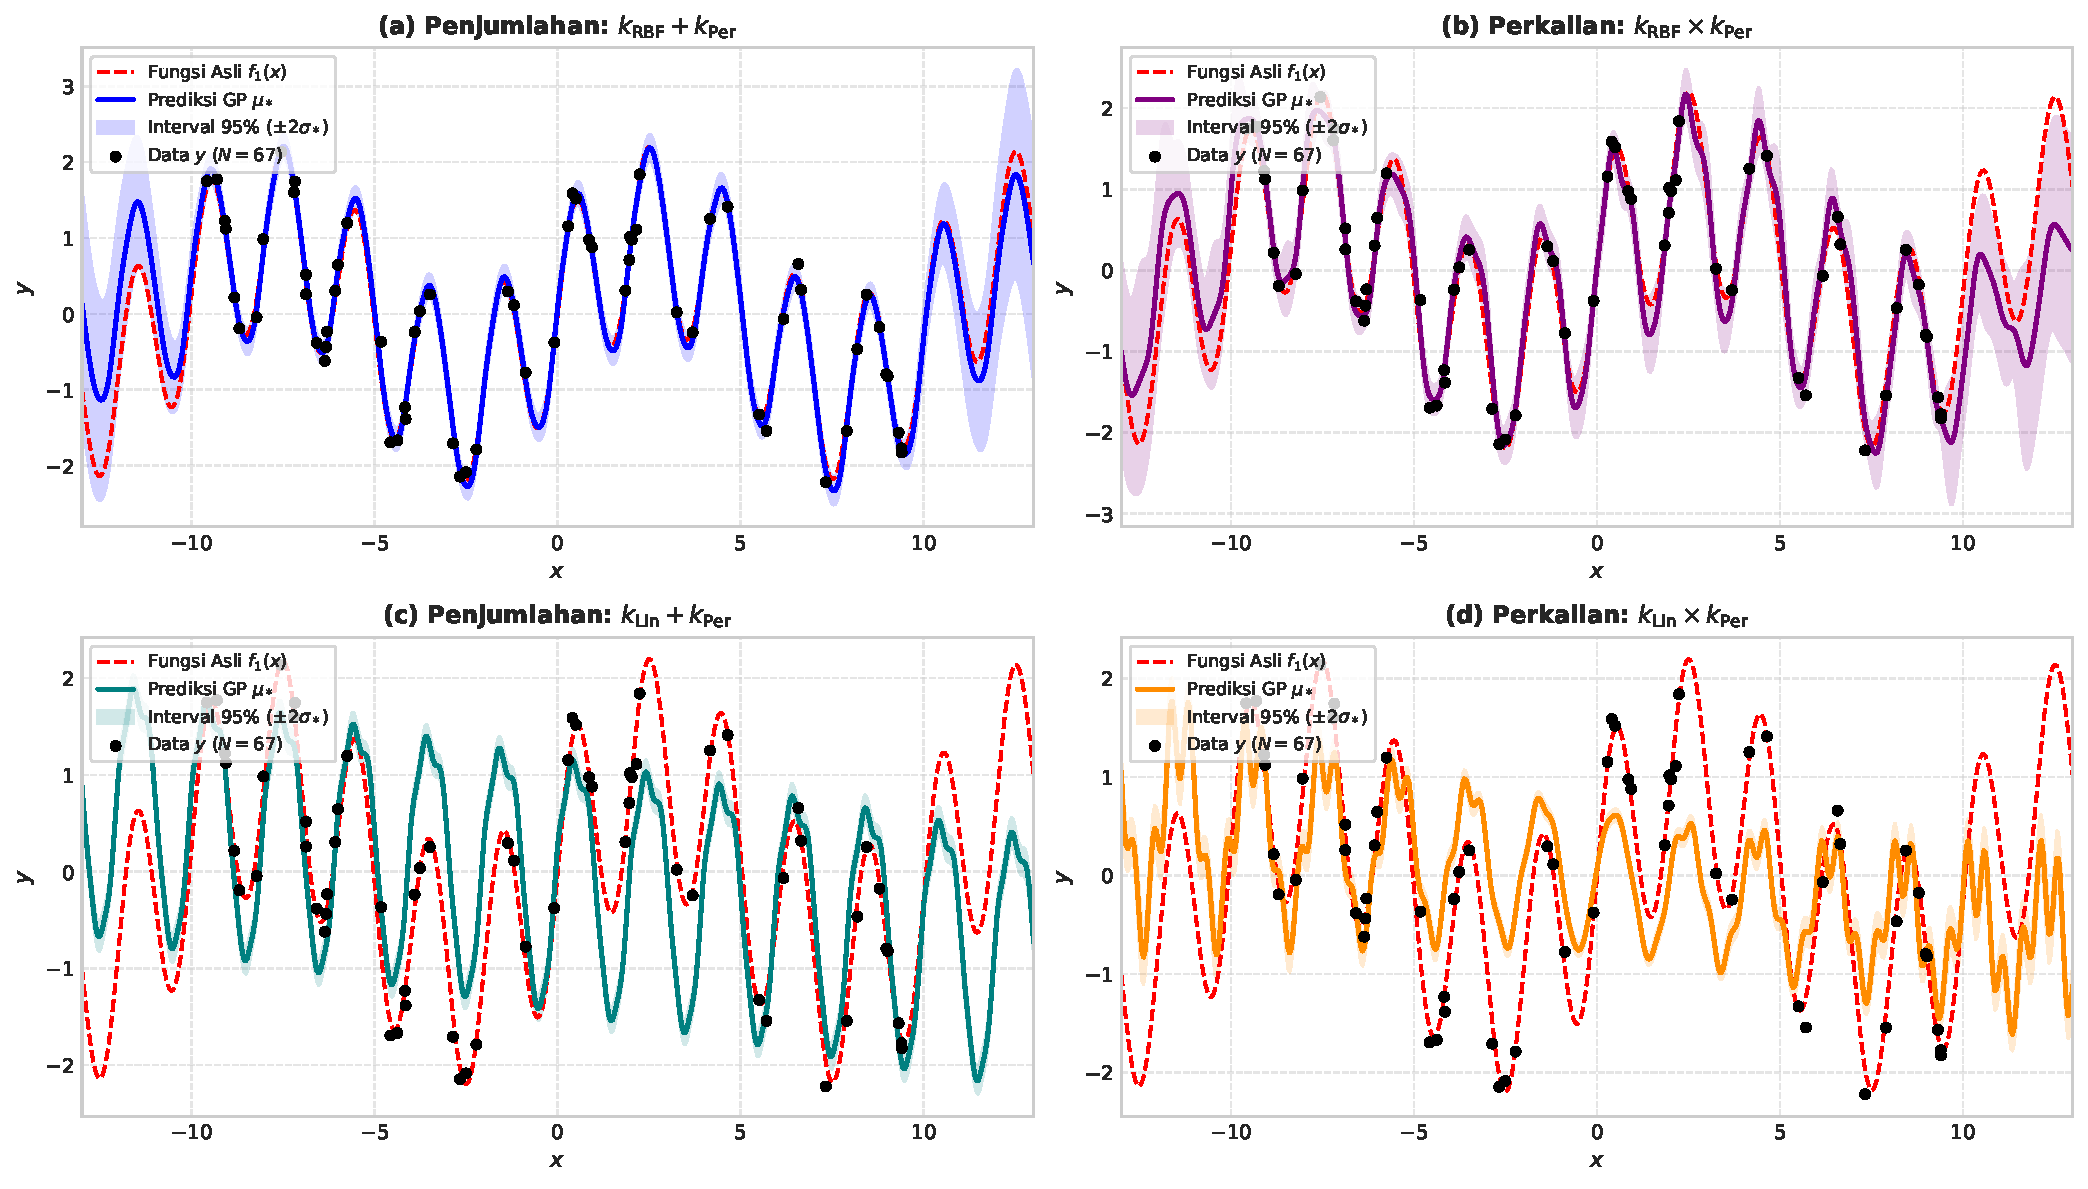
\includegraphics[width=\textwidth]{kernel_fitting_f1.pdf}
\caption{Hasil \textit{fitting} Gaussian Process Regression pada fungsi asli $f_1(x)$ \eqref{eq:true_function_1}: (a) $k_{\mathrm{RBF}} + k_{\mathrm{Per}}$; (b) $k_{\mathrm{RBF}} \times k_{\mathrm{Per}}$; (c) $k_{\mathrm{Lin}} + k_{\mathrm{Per}}$; (d) $k_{\mathrm{Lin}} \times k_{\mathrm{Per}}$.}
\label{fig:kernel_fitting_f1}
\end{figure}

\subsection{Eksperimen 2}
\label{subsec:eksperimen_2}

\noindent Fungsi asli yang digunakan:
\begin{equation}
f_2(x) = 0{,}2 x \sin\left(\frac{2\pi x}{2{,}0}\right) \label{eq:true_function_2}
\end{equation}
\noindent dengan $N = 67$ titik data observasi $y_i = f_2(x_i) + \varepsilon_i, \; \varepsilon_i \sim \mathcal{N}(0, 0{,}15^2)$ pada rentang $x \in [-10, 10]$.

\begin{figure}[H]
\centering
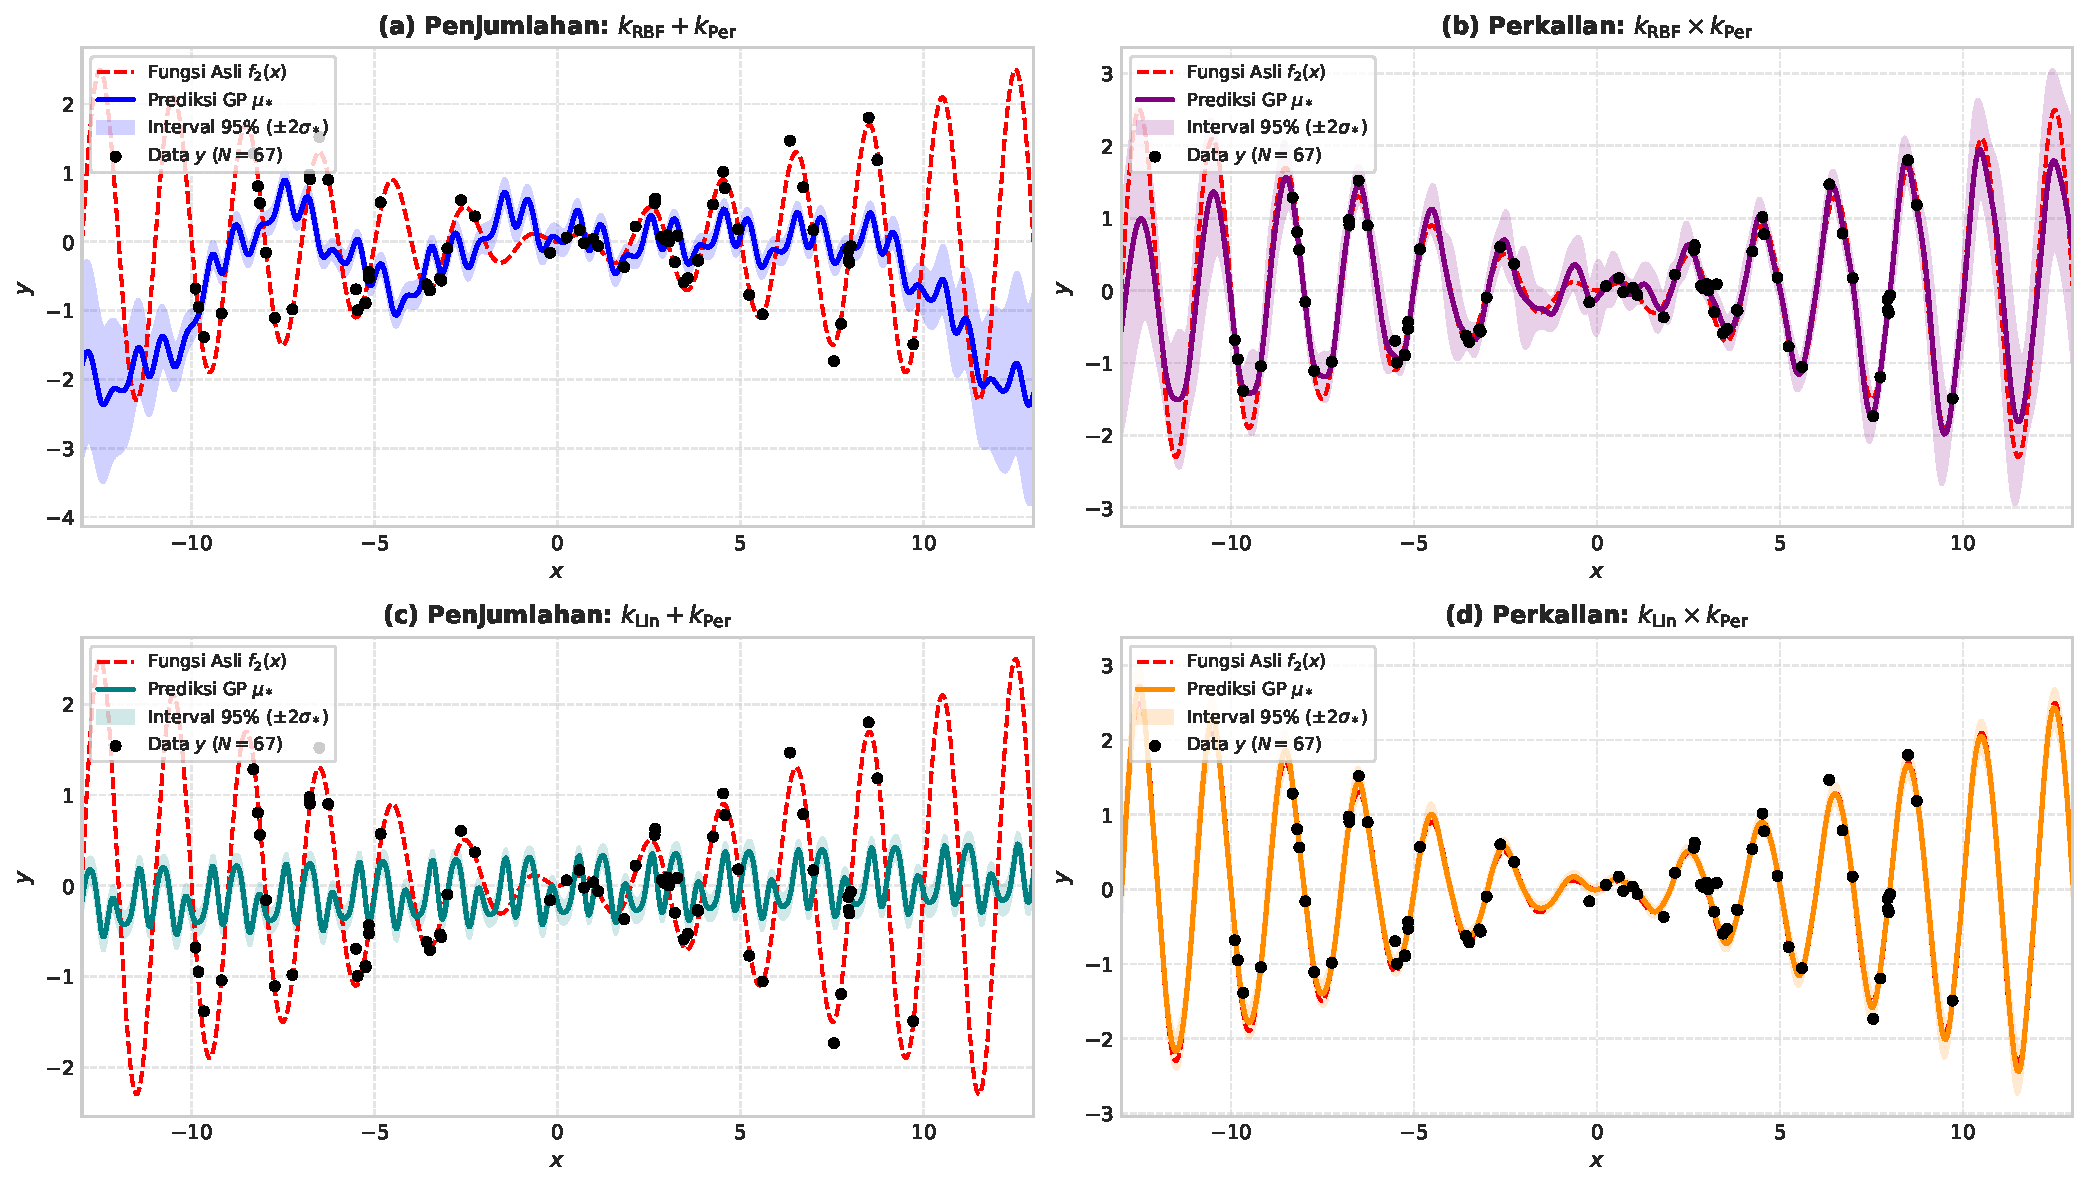
\includegraphics[width=\textwidth]{kernel_fitting_f2.pdf}
\caption{Hasil \textit{fitting} Gaussian Process Regression pada fungsi asli $f_2(x)$ \eqref{eq:true_function_2}: (a) $k_{\mathrm{RBF}} + k_{\mathrm{Per}}$; (b) $k_{\mathrm{RBF}} \times k_{\mathrm{Per}}$; (c) $k_{\mathrm{Lin}} + k_{\mathrm{Per}}$; (d) $k_{\mathrm{Lin}} \times k_{\mathrm{Per}}$.}
\label{fig:kernel_fitting_f2}
\end{figure}

% =========================================================================
% DAFTAR PUSTAKA
% =========================================================================
\begin{thebibliography}{99}

\bibitem{rasmussen2006gaussian}
Rasmussen, C.~E., \& Williams, C.~K. (2006). \textit{Gaussian Processes for Machine Learning}. MIT Press, Cambridge, MA.

\end{thebibliography}

\end{document}
